\documentclass[10pt,fleqn,% ===> this file was generated automatically by noweave --- better not edit it
% linksbündige, abgesetzte Formeln
reqno,a4paper]{article}
\usepackage[utf8]{inputenc}
%\usepackage{amsmath}
\usepackage{amsfonts}
\usepackage{amssymb}
%\usepackage{ngerman}
\usepackage[german, english]{babel}
\usepackage{graphicx}
\usepackage{caption}
\usepackage{subcaption}
\usepackage{hyperref}
\usepackage{natbib}% bibliography style for support for urls in the bibliography
%\usepackage{noweb}
\pagestyle{plain}
%\noweboptions{shift,german,smallcode,longchunks}%smallcode,longchunks
\usepackage[dvipsnames]{xcolor}
\usepackage{comment}
\usepackage{geometry}
%\pagestyle{noweb}\noweboptions{}
\geometry{a4paper, portrait,left=2.5cm, right=2.5cm, top=2cm, bottom=2cm}
\usepackage[T1]{fontenc}
\usepackage[tbtags, % Platzierung der Formel-Tags;% es gibt auch centertags
sumlimits,
% Platzierung der Summationsgrenzen
% (oberhalb/unterhalb)
intlimits,
% Platzierung der Integrationsgrenzen
% (oberhalb/unterhalb)
namelimits]
% Platzierung der Grenzen
% (oberhalb/unterhalb) bei Funktionen
{amsmath}

\usepackage{icomma}% für die richtige Kommadarstellung in Formeln und in Texten
\usepackage[toc,page]{appendix}
\usepackage{listings}% TXT Dateien in LaTeX einbinden

% Farbige Formeln richtig einfärben über die group Umgebung
\def\mathcolor#1#{\@mathcolor{#1}}
\def\@mathcolor#1#2#3{%
        \protect\leavevmode
        \begingroup\color#1{#2}#3\endgroup
}
%\newcommand{\na}{\mathcolor{blue!50!black}{a}}
\newcommand{\nx}{\mathcolor{gray}{x}}
\newcommand{\nnx}{\mathcolor{green!50!black}{x}}
%\newcommand{\nx}{\mathcolor{cyan!70!black}{x}}
\newcommand{\ny}{\mathcolor{gray}{y}}
%\newcommand{\nz}{\mathcolor{green!30!black}{\textit{z}}}
%\newcommand{\nA}{\mathcolor{green!50!black}{A}}
\newcommand{\nw}{\mathcolor{gray}{w}}
%\newcommand{\nW}{\mathcolor{gray}{W}}
\newcommand{\nt}{\mathcolor{gray}{t}}
\newcommand{\ntau}{\mathcolor{gray}{\tau}}
\newcommand{\nW}{\mathcolor{brown!70!black}{W}}
\newcommand{\neta}{\mathcolor{cyan!70!black}{\eta}}
\newcommand{\nnu}{\mathcolor{cyan!70!black}{u}}
\newcommand{\nsin}{\mathcolor{blue!70!black}{\sin}}
\newcommand{\ncos}{\mathcolor{blue!70!black}{\cos}}
\newcommand{\ntan}{\mathcolor{blue!70!black}{\tan}}
\newcommand{\narctan}{\mathcolor{blue!70!black}{\arctan}}
\newcommand{\ncosh}{\mathcolor{blue!70!black}{\cosh}}
\newcommand{\nsinh}{\mathcolor{blue!70!black}{\sinh}}
\newcommand{\nexp}{\mathcolor{blue!70!black}{\exp}}
\newcommand{\nf}{\mathcolor{blue!70!black}{f}}
\newcommand{\nni}{\mathcolor{red!70!black}{i}}
\newcommand{\nm}{\mathcolor{red!70!black}{m}}
\newcommand{\nh}{\mathcolor{blue!70!black}{h}}
\newcommand{\nA}{\mathcolor{blue!70!black}{A}}
\newcommand{\nV}{\mathcolor{blue!70!black}{V}}
\newcommand{\nxi}{\mathcolor{blue!70!black}{\xi}}
\newcommand{\dif}{\mathrm{d}}
\newcommand{\ndelta}{\mathcolor{blue!70!black}{\delta}}
\newcommand{\na}{\mathcolor{blue!70!black}{a}}
\newcommand{\nb}{\mathcolor{blue!70!black}{b}}
\newcommand{\nN}{\mathcolor{blue!70!black}{N}}
\newcommand{\nphi}{\mathcolor{blue!70!black}{\phi}}
\newcommand{\nr}{\mathcolor{blue!70!black}{r}}
\newcommand{\nT}{\mathcolor{blue!70!black}{T}}
\newcommand{\nln}{\mathcolor{blue!70!black}{\ln}}
\newcommand{\nD}{\mathcolor{green!50!black}{D}}
\newcommand{\nz}{\mathcolor{brown!70!black}{z}}
\newcommand{\nF}{\mathcolor{blue!70!black}{F}}
\newcommand{\mA}{\mathcolor{green!50!black}{A}}
\begin{document}\selectlanguage{english}
%@

\begin{titlepage}

\begin{center}


% Oberer Teil der Titelseite:

\begin{minipage}{0.57\textwidth}
\begin{flushleft}\large
\begin{center}
Universität Potsdam\\
Mathematisch-Naturwisssenschaftliche Fakultät\\
Institut für Physik und Astronomie\\
\end{center}
\end{flushleft}
\end{minipage}
\hfill
\begin{minipage}{0.42\textwidth}
\begin{flushright}
\begin{center}

\includegraphics[width=0.55\textwidth]{logo.png}\\ 
\end{center}
\end{flushright}
\end{minipage}
\vfill
\vspace*{0.5cm}
\textsc{\large Computational Physics}\\[0.5cm]


% Title
%\newcommand{\HRule}{\rule{\linewidth}{0.5mm}}
%\HRule \\[0.4cm]
{ \Huge \bfseries Stochastic Resonance}\\[0.4cm]

%\HRule \\[1.5cm]
\vspace*{2.5cm}

% Author and supervisor
\begin{minipage}{0.45\textwidth}
\begin{flushleft} \normalsize 
Author: Alexander Putz\\ 
Matrikel-No: 763265\\
Author: Christian Gößl\\
Matrikel-No.:762627

\end{flushleft}
\end{minipage}
\hfill
\begin{minipage}{0.45\textwidth}
\begin{flushright} \normalsize 
\begin{flushleft}
corrector: Prof. Dr.~Arkady Pikovsky\\
\end{flushleft}
\end{flushright}
\end{minipage}

\vfill
{\normalsize  19.07.2019}
\vspace*{4.5cm}
% Unterer Teil der Seite


\end{center}

\end{titlepage}
\tableofcontents
\newpage
\citestyle{nature}

\section{Introduction}
When taking a look at phenomena like weather, biological systems, etc., one does always have to take unknown, not determinable quantities into account. This is usually addressed by adding a statistical part into the equations, which seem to represent the real behavior very well.
We want to investigate a statistical system, that describes a random moving particle with only two states. The hopping rate between these two states is described by the so called Kramers formula. Additionally a periodic force and a white Gaussian noise acts on the particle. This leads to a stochastic differential equation. By carefully tuning noise and driving force, one can observe the phenomena of stochastical resonance.
Applications can be nothing less than our climate with periods of warm and cold states.


%If we want to describe the phenomena like the weather, biological systems etc, then we have to take into account, that the system is also determined by unknown characteristics or states. We have to regard equations that depend on some random parts. But it exists an interesting phenomena the stochastic resonance. We want to investigate a system, that describes a random moving particle in a potential with only two states. The hopping rate between the two states is described by the kramers formula. Additionally a periodic force act on that particle. The reaction leads to the stochastic resonance. A good example is the diapole of the earth. It makes a switch in the polaristion of the magnetic field. So in our world we have physical systems, that seems to be very stable, but these ones could also have a very long switching rate like the climate system with periods of warm and cold states. In our work we want to simulate it and show the main properties of that. 

\section{Stochastic Resonance Equation}
In our generic model we investigate the time evolution of a stochastic variable $ \nx $. 
In our work we want to simulate a particle, that is performing a random walk in a fluid, namely the well known brownian motion.
Here we investigate only the drift in $ \nx $ direction. 
Additionally the particle is moving in a potential $ \nV (\nx) $ and we can switch on a driving force.
It has two minima, where the particle can be located.
These two states are separated trough a potential wall $ \Delta V $. 
The time evolution is described as follows: 
\begin{align}
\nx _{\nt} = - \nV_{\nx} (\nx) + A\ncos (\omega \nt + \phi) + \sigma \nxi(\nt) \label{eq:StRe}
\end{align}
The subscript variable means a derivative $ \nx _{\nt} = \dif \nx/ \dif \nt $.
As usual: $ \nt $ time variable, $ A $ amplitude and $ \omega $ frequency of the oscillator and $ \nxi (\nt) $ as noise, it is the temporal derivative of a Wiener Process.
\begin{align}
	\nxi(\nt) = \frac{\dif \nW}{\dif \nt}
\end{align}
The potential function $ \nV (\nx) $ of the stochastic variable $ \nx $:
\begin{align*}
\nV (\nx) = -\frac{1}{2}\nx ^2 + \frac{1}{4} \nx ^4
\end{align*}
We use an oscillator to get a triggered resonance.
 In our model we work with an additional Gaussian white noise and with the auto-correlation we get
\begin{align}
        \langle \nxi (\nt) \nxi(0) \rangle = 2D \ndelta(\nt)
\end{align}
with $ \sigma $ the noise factor, hence the variance of noise is $ \sqrt{2D} = \sigma $.
 In our investigation we set the initial phase to
 \begin{align*}
	 \phi = 0 \; .
 \end{align*}
We add all relations together and get for our simulation the main equation:
\begin{align}
        \nx _{\nt} =\nx ^3 -\nx + A\ncos (\omega \nt) +  \sqrt{2D} \nxi(\nt) \label{eq:StReq1}
\end{align}
The two minima of the potential function are $ \nx _{\pm} = \pm 1 $ and hence we have $ \Delta V = 1/4 $.


\subsection{Numerical solution method: Euler-Maruyama} \label{CH:EM}
In general, the stochastic differential equation can be expressed in the differential form:
\begin{align}
        \dif \nx = \na(\nt,\nx) \dif \nt + \nb(\nt,\nx )\dif \nW 
        %\dif \nx _{\nt} = \na(\nt,\nx _{\nt}) \dif \nt + \nb(\nt,\nx _{\nt})\dif \nW _{\nt}
\end{align}
The initial value problem is calculated through
\begin{align}
\nx _{\nni+1}=& \nx _{\nni} +\na(\nt _{\nni},\nx _{\nni}) \Delta \nt_{\nni} + \nb(\nt _{\nni},\nx _{\nni}) \Delta \nW _{\nni}
\end{align}
with $  \na(\nt _{\nni},\nx _{\nni})  $ as function for the non-stochastic part
\begin{align*}
\na(\nt _{\nni},\nx _{\nni})= \nx_{\nni}-\nx _{\nni} ^3  + A\ncos (\omega \nt _{\nni})
\end{align*}
and $ \nb(\nt _{\nni},\nx _{\nni}) $ as function for the stochastic part
\begin{align*}
\nb(\nt _{\nni},\nx _{\nni}) = \sqrt{2D}\;.
\end{align*}
For $ \Delta \nW_{\nni}  $ we need a random distributed variable $ \nz_i $. We are using here the normal distribution $ \nF(\mu,q) $, which is white noise, with
\begin{align*}
	\nz_{\nni} & \in \nF(0,1)\\
	\Delta \nW_{\nni}& = \nz_{\nni}\sqrt{\Delta \nt_{\nni}}
\end{align*}
Summing up all equations, we receive:
\begin{align}
\nx _{\nni+1}=& \nx _{\nni} + (\nx_{\nni}-\nx _{\nni} ^3  + A\ncos (\Omega \nt _{\nni}) )\Delta \nt_{\nni} + \nz_{\nni} \sqrt{2D \Delta \nt_{\nni}} \label{eq:num}
\end{align}

\begin{comment}

	$ \dif\nW_{\nni} = \nx_{\nni}\sqrt{\Delta t} \quad \nx_{\nni} $ of $ \nx_{\nni} = \nN(0,1) $ \\
	or $ \dif\nW _{\nni} = \nx_{\nni} \quad \nx_{\nni}=\nN(0,\sqrt{\Delta \nt}) $ 
	
	equivalent stochastic equation solving method
	$ \dif\nW_{\nni} = \sqrt{2} z_{\nni} \sqrt{\Delta t} $ with $ \nx_{\nni} = \nN(0,1) $
	
	because of $ \langle e(t)e(t')\rangle = 2\delta (t-t')$ here $D$ out of the integral and set to $ D = \sigma^2$
$ 	\sqrt{2 \sigma\Delta t}() $
\end{comment}


\subsection{Kramers formula - Kramers rate} \label{CH:kramers}
Kramers formula is used to give a time scale for the noise induced hopping. For the switching rate $ \nr_{\mathrm{K}} $ we have the equation
\begin{align}
	\nr_{\mathrm{K}}(\nD) = \frac{1}{\sqrt{2}\pi}\nexp\left(- \frac{\Delta V}{\nD} \right)\; . \label{eq:kramer}
\end{align}
With some rearrangements and $ \nr_{{\mathrm{K}}} = 1 / \nT_{{\mathrm{K}}} $ we get
\begin{align}
	\nln (\nT_{\mathrm{K}})(\nD) = \Delta V \frac{1}{\nD} + \nln(\sqrt{2}\pi)
\end{align}
Further we insert the preset values and the equation that we want to prove
\begin{align}
\nln (\nT_{\mathrm{K}})(\nD)\approx 0.25\left( \frac{1}{\nD} \right) + 1.49130 \; . \label{eq:lin-logT_K}
\end{align}

\subsection{Stochastic resonance}
The main aspect of our work is the stochastic resonance. The resonance comes into account, when we turn on the driving force. It's evolving in time and the hopping between the states can be described by the Kramer formula. Naturally we get a resonance, when the frequency of Kramer and the driving force are in resonance. Later on, we will see, that our first impression is not entirely true. 
The particle is moving randomly, but with the periodic force we want to investigate how the random process is depending on the frequency $ \omega $ and noise strength $ D $. 
%In our investigation 

For that we study the phase and amplitude of the time evolution. So we want to know the response of the system, hence we need a Fourierstransformation - FFT, to find the phase and amplitude of the signal at frequency of the driving force $ \omega $. We get from the FFT the Fouriercoefficents $ a_k, b_k $ and can compute the amplitude $ A $ and phase $ \phi $. 
\begin{align*}
	A = \sqrt{a_k^2+b_k^2} \quad \phi = \narctan\left(\frac{a_k}{b_k}\right)
\end{align*}

In the paper \cite{gammaitoni_stochastic_1998}, we find the equation for the stochastic resonance.

\begin{align} \label{eq:phi}
\bar{\nphi}(\nD)= \narctan\left(\frac{\omega}{2 \nr_{\mathrm{K}}(\nD)}\right)
\end{align}

The Maximum resonance $ \bar{\phi}_{\mathrm{max}} $ is reached at $\omega=\pi \nr_{\mathrm{K}}$. %(I will reference on that in response examination chapter)
\begin{align}
	\bar{\nphi}_{\mathrm{max}}(\omega=\pi \nr_{\mathrm{K}}) = \narctan \left(\frac{\pi}{2}\right)
\end{align}
\newpage
\section{Numerical investigation of our stochastic DGL}

\subsection{Setup the simulation} \label{CH:Data_generation}
The data is generated via numerical solution(see chapter \ref{CH:EM}) of the stochastical differential equation \eqref{eq:StReq1}. 
This is done via the \texttt{set\_Data()} function. In this function the data are calculated for a given set of parameters: frequency of the driving force $ \omega $, amplitude of the driving force $ A $, noise intensity $ D $, time step $ \Delta \nt $, amount of iteration $ N $, which were transferred during function \texttt{call()}. 
Later we decided to calculate time step with
\begin{align*}
	\Delta \nt = \frac{2\pi L}{N \omega} 
\end{align*}
Because for the computation of nonlinear dependency of the amplitude $ A $, we set the duration of simulation to $ T\cdot L $, where $ T $ describes the period of the driving force and the factor $ L $ gives us a time evolution until the period ended.  
In our investigations we often use a mean of a physical quantity, due to get better stochastic relevant results. 

 At first \texttt{init()} function is initializing streams for output. The first call of \texttt{output()} sets the boundary conditions at $\nt_0=0$ and $ \nx (\nt_{0})=0 $. After that, \texttt{N} iterations of the SDE are done and stored in the vector \texttt{x}. 
The received data can now be used for further investigations.
In graphic \ref{pic:data}, an exemplary set of data is shown.

\begin{figure}[htpb]
	  \begin{minipage}[b]{0.5\linewidth}
		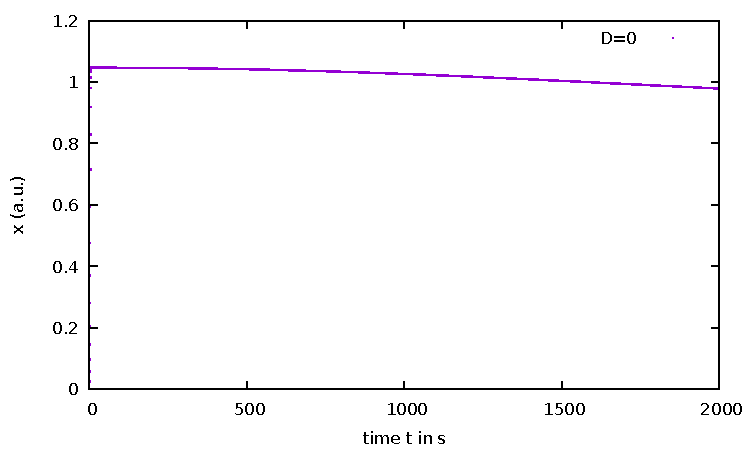
\includegraphics[width=\linewidth]{gnuplot_pictures/final_pictures/Data_plot_D0.pdf} 
	\end{minipage} 
	  \begin{minipage}[b]{0.5\linewidth}
	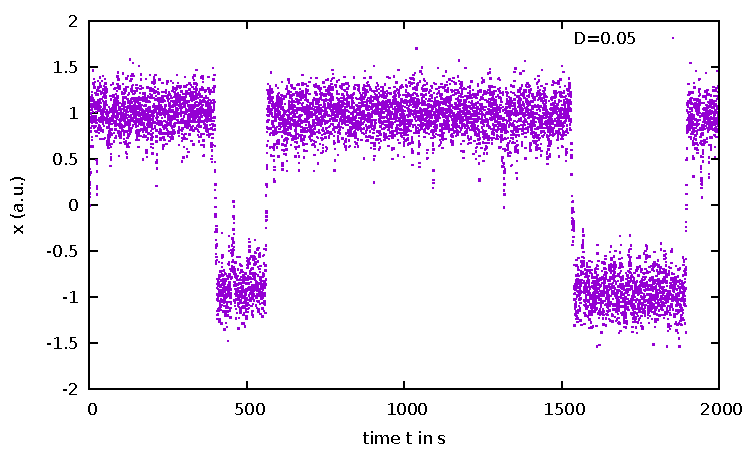
\includegraphics[width=\linewidth]{gnuplot_pictures/final_pictures/Data_plot_D0p05.pdf} 

	\end{minipage} 
	  \begin{minipage}[b]{0.5\linewidth}
	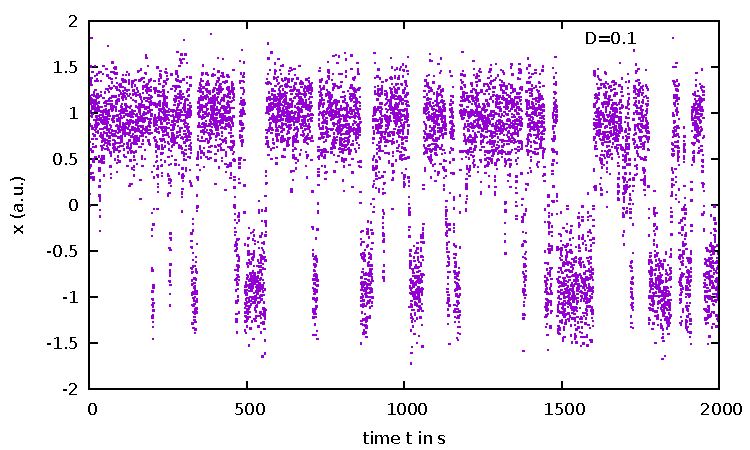
\includegraphics[width=\linewidth]{gnuplot_pictures/final_pictures/Data_plot_D0p1.pdf} 
\end{minipage} 
	  \begin{minipage}[b]{0.5\linewidth}
	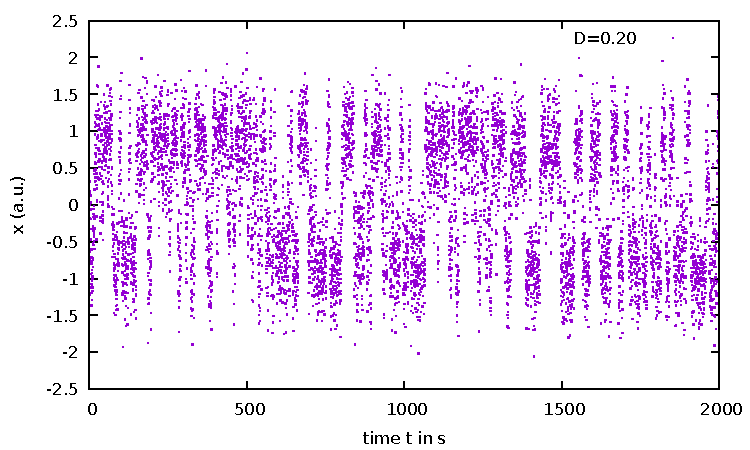
\includegraphics[width=\linewidth]{gnuplot_pictures/final_pictures/Data_plot_D0p2.pdf} 
\end{minipage} 
\caption{The data was gathered for an amplitude $A= 0.1$ and a frequency $\omega=0.001$. The graphs, display data for different noise ranging from $0$ to $0.25$. Between $D=0,05$ and $D = 0.1$, one can see a oscillation of the response signal. For $D= 0$, there is hardly an oscillation visible}
\label{pic:data}
\end{figure}

\newpage

\subsection{Verification of the Kramers formula}\label{sec:kramer}
Here we want to prove the Kramers formula. The Kramers formula describes the switching rate $ \nr_{\mathrm{K}} $ between the two potential states. 
In our simulation we have the states up and down. 
From the amount of states $ n_{\mathrm{K}} $ we can calculate the period $ \nT_{\mathrm{K}} $. We calculated the mean value of the $  \nln \bar{\nT}_{\mathrm{K}} $ for specific times $ \texttt{M} $
\begin{align*}
	\nln \bar{\nT}_{\mathrm{K}} = \frac{N\Delta \nt M}{n_{\mathrm{K}}} \; .
\end{align*}
 So we need an algorithm, that can detect these states of our simulation. 
The program detects and counts the changings with our predefined rules in the function \texttt{kramer()}.
The principle goes like this: Whenever $ \nx_{\nni} $ is in up or down state, the function checks, whether there was a transition from the opposite state or $ \nx_{\nni} $ remains in the state it was before. After more calculations the values goes up and we have a up state. 
Then the procedure starts again as before. We indicate the states with the Boolean variable \texttt{mess} and when the values either for up $ \nx_{\nni} > 0.99 $ or down $ \nx_{\nni}  < -0.99 $. At the beginning it  is set to \texttt{false}. It changes to \texttt{true}, when the next down state is reached. Our convention for the states is up with \texttt{mess = false} and down with \texttt{mess = true}. You can see the whole code in the appendix. For the verification of Kramer formula we use the equation \eqref{eq:lin-logT_K}. It is fitted to our calculated values $ \nln (\nT_{\mathrm{K}})(\nD) $. 
\begin{align*}
	\nln (\nT_{\mathrm{f}})(\nD)= a\left( \frac{1}{\nD} \right) + b
\end{align*}
%with $ f(\nnx) = \nln (\nT_{\mathrm{K}})(\nD) $ and $ \nnx = 1/\nD $. 
 
\begin{align*}
L = 30\,, N = 10^6\,, A = 0\,, \omega=0.5\,, D_{\mathrm{init}} = 0.1\,,  D_{\mathrm{end}} = 0.5\,, M = 20
\end{align*}
See the figure \ref{pic:T_K} for the results.
\begin{figure}[htp!]
	\begin{center}
		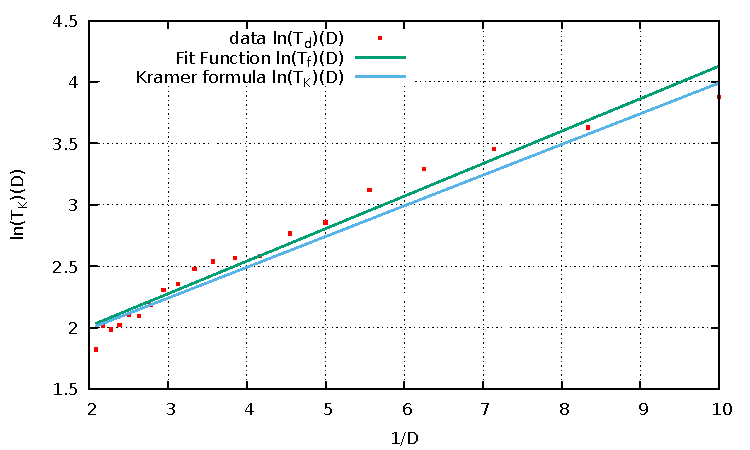
\includegraphics[width=\linewidth]{../sourcecode_output_Data/plotting-T_K-docu-2.pdf}%[scale=0.5]
		\caption{Comparison between the fitting function $ \nln(\nT_{\mathrm{f}})(\nD) $ and the calculated function $ \nln(\nT_{\mathrm{K}})(\nD) $. red squares: the calculated values, green line: fit function, blue line: Kramer formula. The slope of the fit function has a good agreement with the Kramer formula. It is slightly shifted upwards.}
		\label{pic:T_K}
	\end{center}
\end{figure}

For our fit function we get the following parameters:

\begin{align*}
\nln(\nT_{\mathrm{f}})(\nD) \approx 0.26454\left( \frac{1}{\nD}\right) + 1.48301 \quad \nln (\nT_{\mathrm{K}})(\nD) \approx 0.25\left( \frac{1}{\nD} \right) + 1.49130
\end{align*}
\begin{comment}
	a               = 0.264537         +/- 0.01198      (4.53%)
	b               = 1.48301          +/- 0.05692      (3.838%)
\end{comment}
 Our result gives us a good agreement with the predicted model of the Kramer formula. 
\newpage
\subsection{Response examination in dependence of noise} \label{sec:CH_response}
The beforehand gathered data (see section \ref{CH:Data_generation}) are Fourier-Transformed at the periodic driving frequency $\omega$. The Fourier-Transformation is done via the function \texttt{FFT()}.% For more information on how to perform a Fourier Transformation see the literature. 
%source for literature?
Varying the noise intensity $D$ and determining the output amplitude of the Fourier components, one gets in figure \ref{pic:ampl_phase_wo_errorbars} the shown trend.
As one can see, there is a maximum amplitude at a noise of about $D = 0.04$. This is called "stochastical resonance". At this noise strength, the Kramers rate $\nr_{K}$ and the periodic force are in resonance. The amplitude even gets stronger than without noise.
If the noise gets even stronger, the switching is driven by the noise and the Kramers rate gets smaller. Therefore the amplitude at the periodic forcing $\omega$ gets smaller.
Additionally one can observe a drop in phase shift of the $\nsin$ and $\ncos$ components.
Out of resonance the phase shift is stable at $\pi/2$, but in resonance the phase shift gets reduced to about $0.2$.
Taking a closer look at the Fourier coefficients $a_k$ and $b_k$ in figure \ref{pic:phase} unveils the phase shifts shape.
The $\ncos$ component $b_k$ shows a peak at the rising flank of the amplitude. This is due to the input signal, which is also a $\ncos$ function. In contrast to that, the $\nsin$ component follows the amplitudes shape.
As already explained in chapter \ref{CH:kramers}, the matching condition(resonant case) is $\omega=\pi \nr_{K}$. Inserting the condition in equation \eqref{eq:phi} yields
\begin{align}
\bar{\phi}_{\mathrm{max}}=\narctan\left(\frac{\pi}{2}\right) = 1
\end{align}
This means, there is a fixed phase shift in the resonant case, which can be confirmed with figure \ref{fig:var_amp}. The maximum response amplitude is always at a phase shift of $1$ (Caution, do not mix with the phase shifts minimum).


To get statistical data, this analysis was performed $10$ times using the function \texttt{Fourier\_task()} and averaged. The function does also return the amplitudes and phase shifts variance. This can be seen in figure \ref{pic:ampl_phase_with_errorbars} .
Before reaching the resonant state, the variance for both amplitude and phase shift is nearly not existent compared to the variance at higher noise rates. This can be ascribed to the fact, that the oscillation is a statistical process and the variance will get smaller with increasing iteration numbers.


\begin{figure} 
	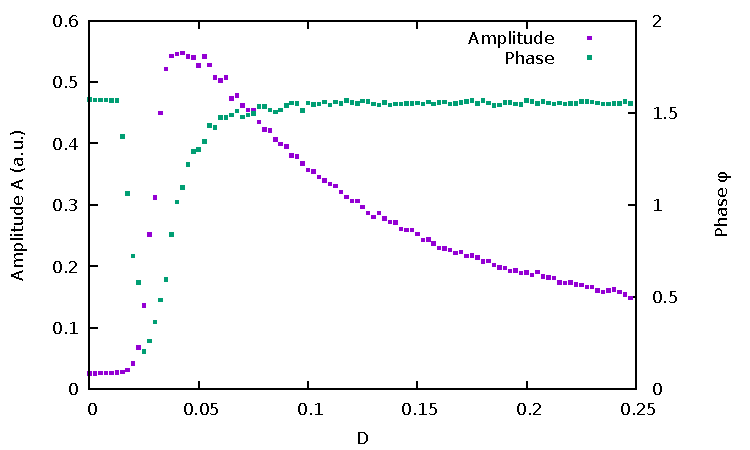
\includegraphics[width=\linewidth]{gnuplot_pictures/final_pictures/ampl_phase_wo_errorbars-1.pdf}
	\caption{amplitude-phase plotted against noise intensity $D$ for $A=0.1$ and $\omega=0.001$}
	\label{pic:ampl_phase_wo_errorbars}
\end{figure}

\begin{figure} 
	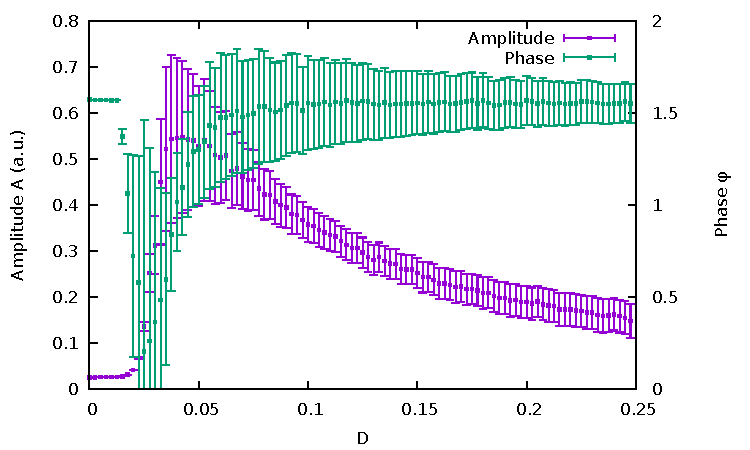
\includegraphics[width=\linewidth]{gnuplot_pictures/final_pictures/ampl_phase_with_errorbars-1.pdf}
	\caption{amplitude-phase plotted against noise intensity $D$ for $A=0.1$ and $\omega=0.001$ with errorbars (variance). The number of iterations was 10}
	\label{pic:ampl_phase_with_errorbars}
\end{figure}

\begin{figure} 
	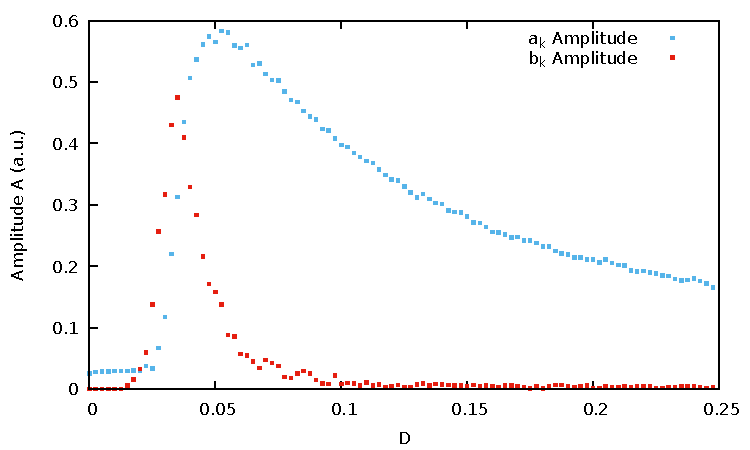
\includegraphics[width=\linewidth]{gnuplot_pictures/final_pictures/phase-.pdf}
	\caption{coefficients $a_k$ and $b_k$ in dependency of noise intensity $D$ for $A=0.1$ and $\omega=0.001$}
	\label{pic:phase}
\end{figure}
\newpage
\subsection{Examine non-linear properties of the signals amplitude $ A $}
In this part we want to inspect the non-linear properties of the signal amplitude $ A_{\mathrm{out}} $. 
For this task the algorithms and functions from chapter \ref{sec:CH_response} can be taken. The input signals amplitude $A_{\mathrm{in}}$ was varied from $0.03$ to $2.0$ as can be seen in figure \ref{fig:var_amp}. Also for comparison all plots can be seen in figure \ref{fig:all-A-D}.
The systems amplitude rises with increasing signal amplitude. The increase is not linear. Increasing the signals amplitude from $A=0.03$ to $A=0.1$ (factor of about 3), increases the systems amplitude by a factor of about $2$. A further increase of the signals amplitude from $0.1$ to $A=1$ (factor of 10), results in a much smaller increase of about $45\%$. Also, after reaching a certain level, the resonance peak shifts to lower noise intensities with rising signal amplitude. It seems like the peak shifts to "`negative"' noise, which would be nonphysical.

A possible explanation could be, that with a high signal strength the system is not anymore governed by the noise and therefore stochastical resonance occurs no longer. Also, the role of potential diminishes. In the presented case this is somewhere between $A=0.2$ and $A=0.4$.

\begin{figure}[htpb]
	
	\begin{minipage}[b]{0.5\linewidth}
		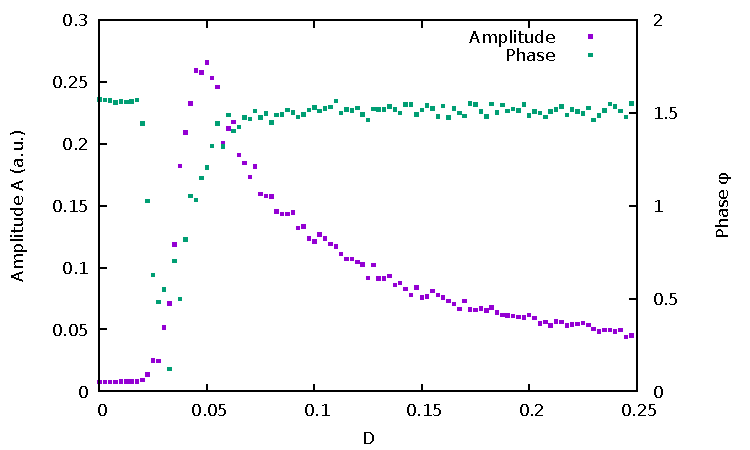
\includegraphics[width=\linewidth]{gnuplot_pictures/final_pictures/ampl_0p03_phase.pdf}
		\subcaption{signal amplitude $A=0.03$} 
	\end{minipage} 
	\begin{minipage}[b]{0.5\linewidth}
		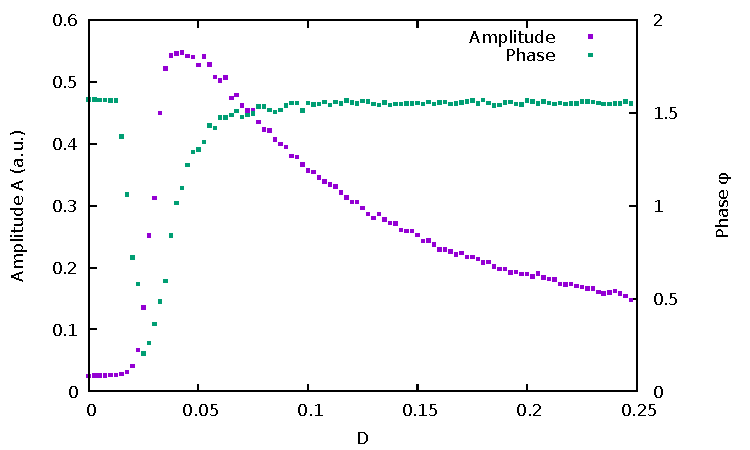
\includegraphics[width=\linewidth]{gnuplot_pictures/final_pictures/ampl_0p1_phase.pdf} 		
	\subcaption{signal amplitude $A=0.1$}
	\end{minipage} 

	\begin{minipage}[b]{0.5\linewidth}
		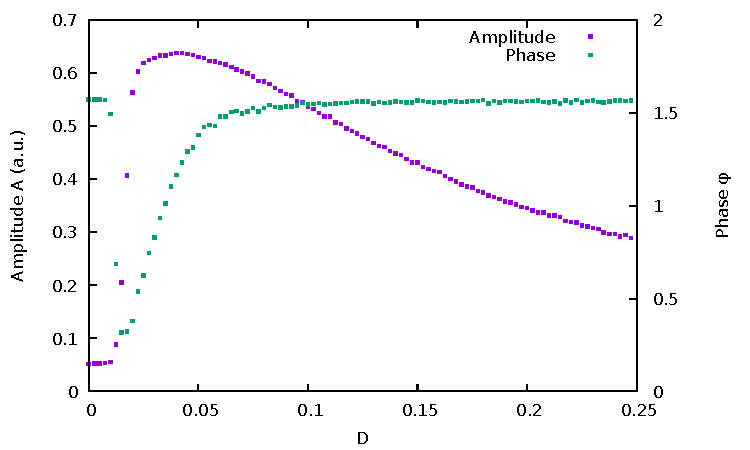
\includegraphics[width=\linewidth]{gnuplot_pictures/final_pictures/ampl_0p2_phase.pdf}
		\caption{signal amplitude $A=0.2$} 
	\end{minipage} 
	\begin{minipage}[b]{0.5\linewidth}
		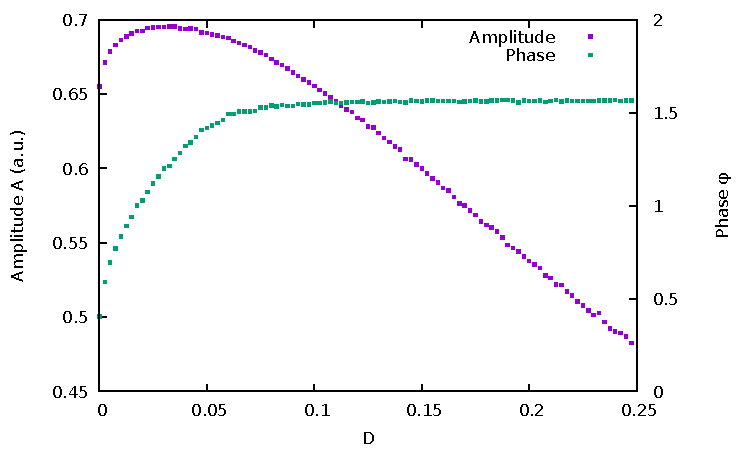
\includegraphics[width=\linewidth]{gnuplot_pictures/final_pictures/ampl_0p4_phase.pdf} 
		\subcaption{signal amplitude $A=0.4$} 
	\end{minipage} 

	\begin{minipage}[b]{0.5\linewidth}
	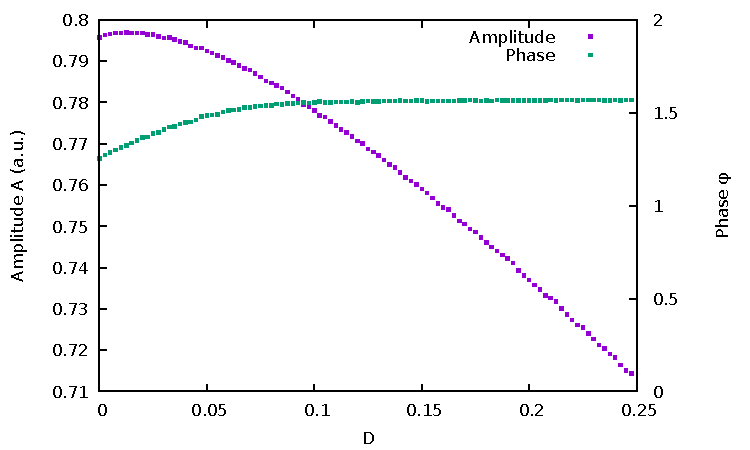
\includegraphics[width=\linewidth]{gnuplot_pictures/final_pictures/ampl_1p0_phase.pdf} 
			\subcaption{signal amplitude $A=1.0$} 
	\end{minipage} 
	\begin{minipage}[b]{0.5\linewidth}
	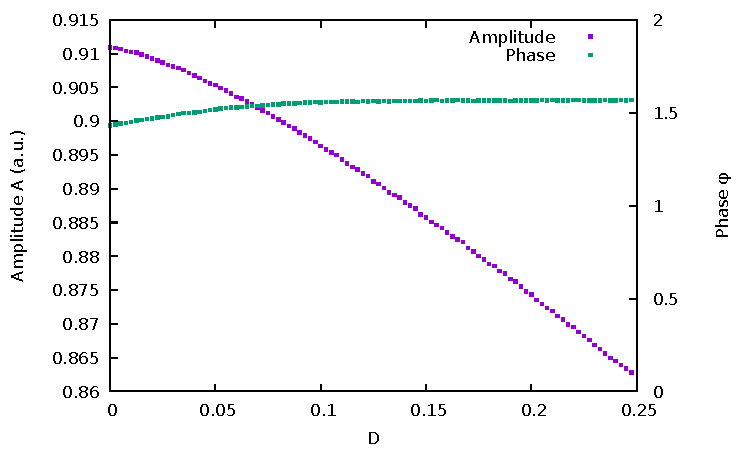
\includegraphics[width=\linewidth]{gnuplot_pictures/final_pictures/ampl_2p0_phase.pdf} 
				\subcaption{signal amplitude $A=2.0$} 
	\end{minipage} 
\caption{Response amplitude for different signal amplitudes}
\label{fig:var_amp}
\end{figure}
\newpage
We put the maxima of all plots together in one plot over the input amplitude see figure \ref{fig:max-AO-AI}.

\begin{figure}[htp!]
	\begin{center}
		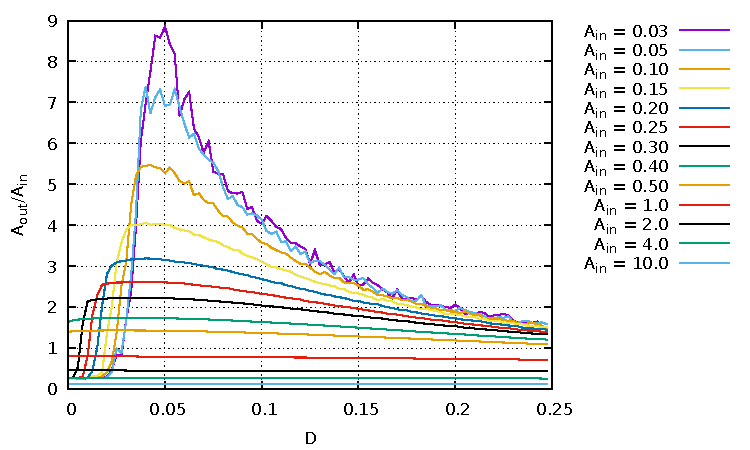
\includegraphics[width=\linewidth]{gnuplot_pictures/plotting-A-D-all.pdf} 
		\caption{The response amplitude of all last plots merged in one plot. The maximum decreases and shifts to the left with the increasing input amplitude} 
		\label{fig:all-A-D}
	\end{center}
\end{figure}

At next we analyze the relation between the maximum of the output amplitude and the input amplitude see figure \ref{fig:max-AO-AI}. We fitting the values to a inverse function and get
\begin{align}
	\nA_{\mathrm{max}}(\mA _{\mathrm{in}}) \approx  \frac{0.864292}{(\mA _{\mathrm{in}}+0.066830)}
\end{align}
As we saw before, it decreases with increasing of the input amplitude. Hence we get a smaller response by a higher input amplitude and the other way around.  
\begin{comment}
Final set of parameters            Asymptotic Standard Error
=======================            ==========================
a               = 0.864292         +/- 0.0216       (2.499%)
b               = 0.0668303        +/- 0.003032     (4.537%
\end{comment}

\begin{figure}[htp!]
	\begin{center}
		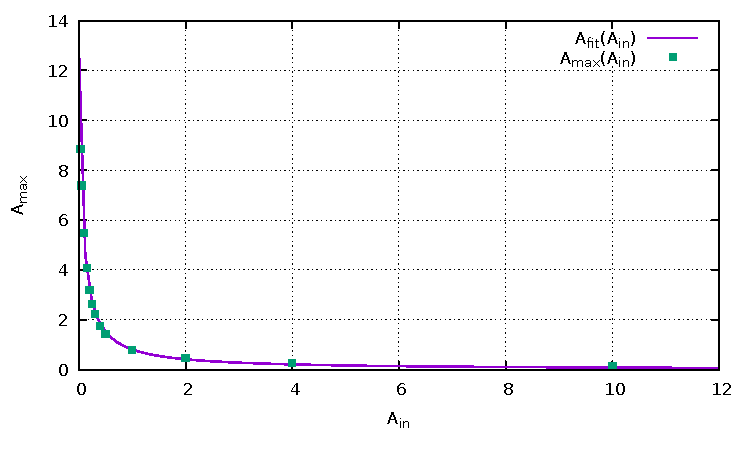
\includegraphics[width=\linewidth]{../plotting-AO-AI.pdf} %gnuplot_pictures/
		\caption{Green squares: maximum values of the output amplitudes. purple line: fit function of the maximum values. The inverse function suits to our maximum values. } 
		\label{fig:max-AO-AI}
	\end{center}
\end{figure}

\newpage
\subsection{Dependency of the time step $ \Delta \nt $}
In this subsection we want to analyze  the simulations behavior on different time steps.
Recap chapter \ref{CH:EM} and equation \ref{eq:num}:
\begin{align*}
	\nx _{\nni+1}=& \nx _{\nni} + (\nx_{\nni}-\nx _{\nni} ^3  + A\ncos (\Omega \nt _{\nni}) )\Delta \nt_{\nni} + \nz_{\nni} \sqrt{2D \Delta \nt_{\nni}}
\end{align*}
As one can see, the statistical part (i.e. noise strength) is dependent on the time step $\Delta \nt$, whereas the deterministic part is not. That will result in different behavior regarding different time steps.
We observed divergent behavior if the time steps are of the size of $0,1$s to $1$s. This can be explained as follows: If the deflection (caused by noise) gets very high, the potentials backward driving force is also very high. If now the time step is also relatively big, the next iteration would yield a position result on the other side of the potential, ignoring the two stable stats. Now the deflection is even higher then before, just on the other side. The change in potential to lower values (i.e. the stable states) is ignored, because of the linear approximation through numeric iteration.
The next iteration is driven backward again but with an even greater elongated position. After several steps, the position reaches infinity(in terms of data storage) and the simulation produces errors.

 

\newpage

\section{Summary}
In our report we investigated the stochastic DGL of a random walking particle in a potential. We computed the solution with the Euler-Maruyama method. In that constellation, we validate the Kramer formula for a specific range of parameters. Than we switched on a oscillating force and we checked the phenomenon of stochastic resonance. In that case we found a relation of the output amplitude and input noise strength. We saw, that the output amplitude is here a nonlinear variable, because the maxima of amplitude function are varying with the input amplitude. All that results depend on the preset time step, because it regulates the accuracy of the computed values and it influences the strength of noise by a factor of $ \sqrt{\Delta \nt} $.  

\newpage
% for bibliography you have to execute 1. pdflatex, 2. biblatex and 2 times pdflatex

\begin{appendices}
	\lstdefinestyle{c++}{
		language=c++,showspaces=false,showstringspaces=false,breaklines=true,numbers=left,frame=single,extendedchars=true,inputencoding=utf8,literate=%
		{Ö}{{\"O}}1 
		{Ä}{{\"A}}1 
		{Ü}{{\"U}}1 
		{ß}{{\ss}}2 
		{ü}{{\"u}}1 
		{ä}{{\"a}}1 
		{ö}{{\"o}}1
	}
	
	\lstdefinestyle{gnuplot}{
		language=gnuplot,showspaces=false,showstringspaces=false,breaklines=true,numbers=left,frame=single,extendedchars=true,inputencoding=utf8,literate=%
		{Ö}{{\"O}}1 
		{Ä}{{\"A}}1 
		{Ü}{{\"U}}1 
		{ß}{{\ss}}2 
		{ü}{{\"u}}1 
		{ä}{{\"a}}1 
		{ö}{{\"o}}1
	}
	\section{Code}
	\lstset{escapechar=@,style=c++}
	\lstinputlisting[caption={Quellcode \texttt{Main.cpp}},label={lst:main.cpp}]{../sourcecode_output_Data/Main-protocol.cpp}
\end{appendices}
\newpage
\nocite{*} % output all references in the bibtex file
\bibliographystyle{plainnat} % support for urls in the bibliography
\bibliography{Exported} % bibtex file without bib extension

\end{document}
